\chapter{Einführung}

\section{Was ist Mathematik?}
Mathematik ist keine Naturwissenschaft. Sie hat aber dennoch viele Anwendungen in den Naturwissenschaften, insbesondere in der Physik, aber auch in anderen Disziplinen, wie etwa den Ingenieur- oder Wirtschaftswissenschaften. Mathematik beschäftigt sich damit, Muster und Strukturen zu erkennen. Sie vermittelt keine interpretationsbedürftigen Ansichten. Sie baut auf objektiven Sachverhalten und logischen Schlussfolgerungen auf.\par

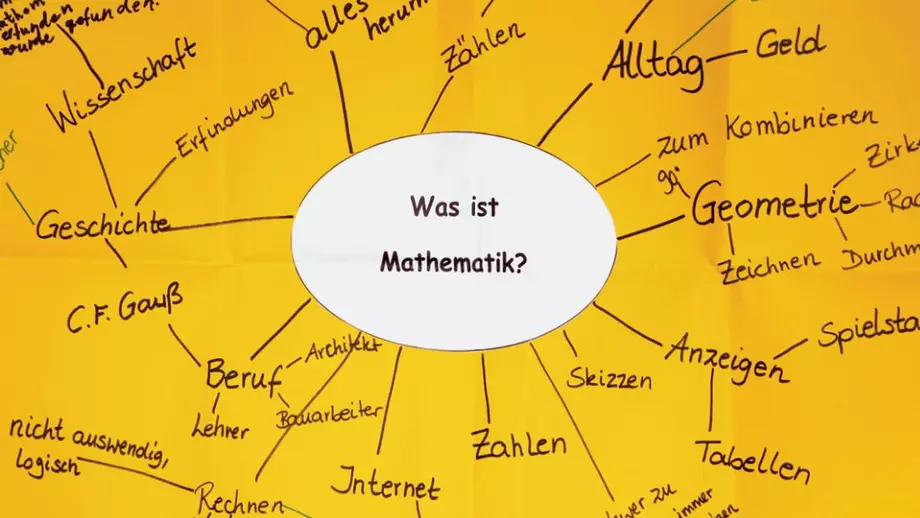
\includegraphics[width=.5\linewidth]{WasIstMathematik}

\section{Warum Mathematik?}
Durch Mathematik können wir viele Dinge in der Welt besser verstehen und begründete Zukunftsprognosen abgeben. Mathematik ist ein Teil unserer Kultur und zugleich die Antwort des Menschen auf die Komplexität der Welt. Uns ist oft nicht bewusst, wie sehr unser Alltag mit Mathematik durchsetzt ist. Mathematik steckt im Mobiltelefon, im Auto, in stabilen Gebäuden, in medizinischen Untersuchungsmethoden, in CDs, in der kühlen Cola, die du trinkst, wenn es dir mal wieder zu heiss wird\ldots
\begin{wrapfigure}{l}{0.5\textwidth}
	\begin{center}
		
\includegraphics[width=0.48\textwidth]{Bergsteigen}
	\end{center}
	\caption{Der Weg ist das Ziel.}
\end{wrapfigure}
Mathematisches Können erwirbt man aber nur durch mathematisches Tun. Wer in der Mathematik voran kommen will, muss üben, sich mit der Materie auseinandersetzen. Bergsteigen lernt man ja auch nicht, indem man Bücher über Berge liest. Wer die Aussicht auf dem Gipfel geniessen will, muss sich anstrengen, muss sich der Aufgabe stellen und selber auf den Berg steigen. Genauso lassen sich die Schönheit und Harmonie der Mathematik nur erkennen, wenn man sich mit ihr beschäftigt.


\begin{figure}
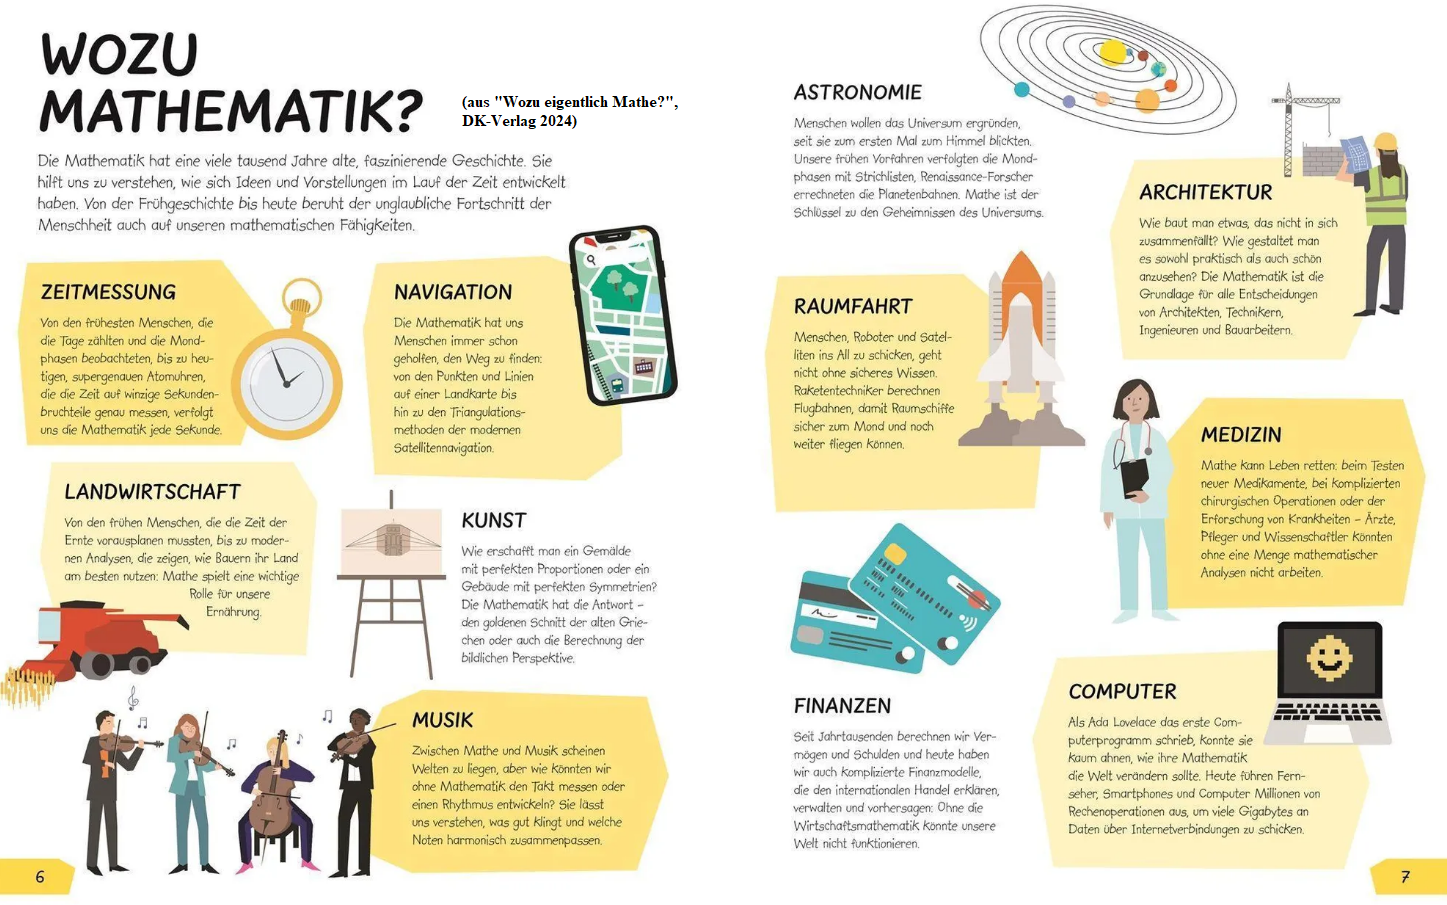
\includegraphics[angle=90,scale=0.65]{WozuMathematik}
\end{figure}
\thispagestyle{empty}
